\label{ch:rotation}

\section{Introduction}

Currently, \castro\ supports contant, solid-body rotation about a fixed
(in space and time) axis in 2D and 3D by transforming the evolution
equations to the rotating frame of reference.

To include rotation you must set
\begin{verbatim}
USE_ROTATION = TRUE
\end{verbatim}
in the {\tt GNUMakefile}.  Rotation can then be enabled via
\begin{verbatim}
castro.do_rotation = 1
\end{verbatim}
in the {\tt inputs} file.  The rotational period must then be set via
\runparam{castro.rotational\_period}.  The rotational period is internally
converted to an angular frequency for use in the source term
equations.

The axis of rotation currently depends on the dimensionality of the
problem and the value of {\tt coord\_sys}; in all cases, however, the
default axis of rotation points from {\tt center}, which is typically
defined in a {\tt Prob\_\$(DIM)d.f90} routine, to the typical ``vertical
direction.''  The vertical direction is defined as follows:
\begin{itemize}
\item 2D
\begin{itemize}
\item {\tt coord\_sys = 0}, (x,y): out of the (x,y)-plane along the ``z''-axis
\item {\tt coord\_sys = 1}, (r,z): along the z-axis
\end{itemize}

\item 3D
\begin{itemize}
\item {\tt coord\_sys} = 0, (x,y,z): along the z-axis
\end{itemize}
\end{itemize}
To change these defaults, modify the {\tt omega} vector in the {\tt
  ca\_rotate} routine found in the {\tt Rotate\_\$(DIM)d.f90} file.


The main parameters that affect rotation are:
\begin{itemize}

\item \runparam{castro.do\_rotation} : include rotation as a forcing
  term (0 or 1; default: 0)

\item \runparam{castro.rotational\_period} : period (s) of rotation
  (default: 0.0)

\item \runparam{castro.rotational\_dPdt} : d(period) / dt for rotation
  (default: 0.0)

\item \runparam{castro.rotation\_include\_centrifugal} : whether to
  include the centrifugal forcing (default: 1)

\item \runparam{castro.rotation\_include\_coriolis} : whether to
  include the Coriolis forcing (default: 1)

\item \runparam{castro.rotation\_include\_domegadt} : whether to
  include the forcing from the time derivative of the rotation
  frequency (default: 1)

\item \runparam{castro.state\_in\_rotating\_frame} : whether state
  variables are measured in the rotating frame (default: 1)

\item \runparam{castro.rot\_source\_type} : method of updating the
  energy during a rotation update (default: 4)

\item \runparam{castro.implicit\_rotation\_update} : for the Coriolis
  term, which mixes momenta in the source term, whether we should
  solve for the update implicitly (default: 1)

\item \runparam{castro.rot\_axis} : rotation axis (default: 3
  (Cartesian); 2 (cylindrical))

\end{itemize}

For completeness, we show below a derivation of the source terms that
appear in the momentum and total energy evolution equations upon
switching to a rotating reference frame.


\section{Coordinate transformation to rotating frame}

\begin{figure}[t]
\centering
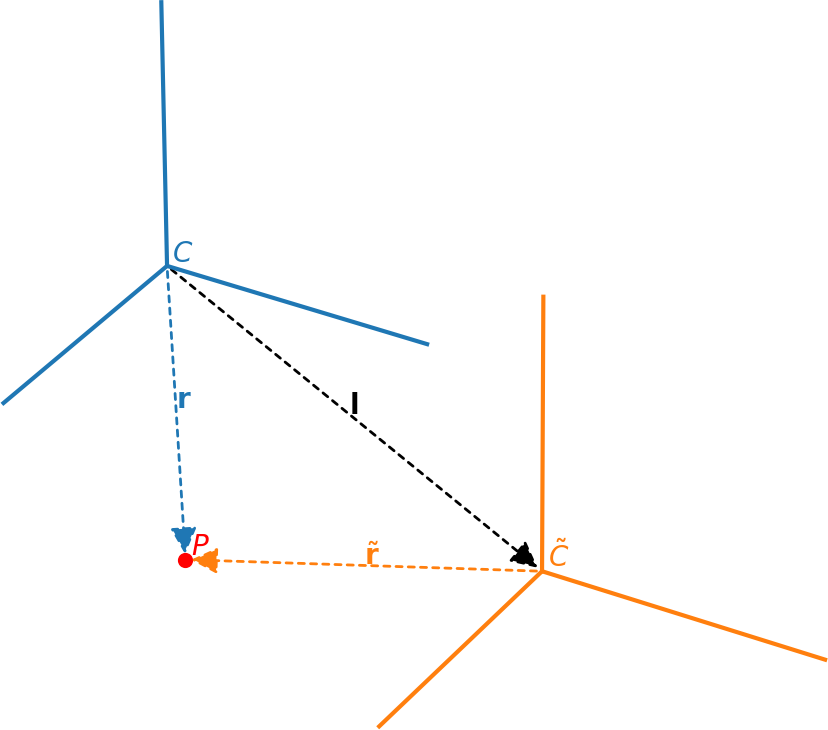
\includegraphics[width=0.5\linewidth]{tframes}
\caption{\label{fig:sec:rot:frames} Inertial frame $C$ and
non-inertial frame $\tilde{C}$.  We consider a fluid element
$P$, whose distance in the two frames is related by 
${\bf r} = \tilde{\bf{r}} + {\bf l}$}
\end{figure}

Consider an inertial reference frame \(C\) and a non-inertial
reference frame \(\widetilde{C}\) whose origins are separated by the
vector \(\boldsymbol{l}\) (see Figure~\ref{fig:sec:rot:frames}).  The non-inertial frame is rotating about the axis
\(\ob\) with a \emph{constant} angular velocity \(\omega\);
furthermore, we assume the \emph{direction} of the rotational axis is
fixed.  Consider a fluid element at the point \(P\) whose location is
given by \(\rb\) in \(C\) and by \(\rbt\) in
\(\widetilde{C}\):
  \begin{equation}
    \rb = \rbt + \boldsymbol{l},
  \end{equation}
or in component notation
  \begin{equation}\label{eq:r}
    r_i\boldsymbol{e_i} = \widetilde{r_i}\widetilde{\boldsymbol{e_i}} + l_i\boldsymbol{e_i},
  \end{equation}
where \(\boldsymbol{e_i}\) and \(\widetilde{\boldsymbol{e_i}}\) are the \(i\)th unit
vectors in the \(C\) and \(\widetilde{C}\) coordinate systems,
respectively.  The total time rate of change of \ref{eq:r} is given by
  \begin{equation}\label{eq:vcomp}
    \frac{Dr_i}{Dt}\boldsymbol{e_i} = \frac{D\widetilde{r_i}}{Dt}\widetilde{\boldsymbol{e_i}} + \widetilde{r_i}\frac{D\widetilde{\boldsymbol{e_i}}}{Dt} + \frac{Dl_i}{Dt}\boldsymbol{e_i},
  \end{equation}
where we have used the fact that the unit vectors of the inertial
frame \(C\) are not moving (or at least can be considered stationary,
and the change in \(\boldsymbol{l}\) gives the relative motion of the two
coordinate systems).  By definition, a unit vector can not change its
length, and therefore the only change of \(\widetilde{\boldsymbol{e_i}}\) with
time can come from changing direction.  This change is carried out by
a rotation about the \(\ob\) axis, and the tip of the unit
vector moves circumferentially, that is
  \begin{equation}\label{eq:etilde-rot}
    \frac{D\widetilde{\boldsymbol{e_i}}}{Dt} = \ob\times\widetilde{\boldsymbol{e_i}}.
  \end{equation}
Plugging \ref{eq:etilde-rot} into \ref{eq:vcomp} and switching back to
vector notation, we have
  \begin{equation}\label{eq:r-dot}
    \frac{D\rb}{Dt} = \frac{D\rbt}{Dt} + \ob\times\rbt + \frac{D\boldsymbol{l}}{Dt}.
  \end{equation}
The left hand side of \ref{eq:r-dot} is interpretted as the velocity
of the fluid element as seen in the inertial frame; the first term on the
right hand side is the velocity of the fluid element as seen by a
stationary observer in the rotating frame \(\widetilde{C}\).  The second
and third terms on the right hand side of \ref{eq:r-dot} describe the
additional velocity due to rotation and translation of the frame
\(\widetilde{C}\) as seen in \(C\).  In other words, 
  \begin{equation}\label{eq:v}
    \vb = \vbt + \ob\times\rbt + \boldsymbol{v_l},
  \end{equation}
where we use \(\boldsymbol{v_l}\) to represent the translational velocity.  

Similarly, by taking a second time derivative of \ref{eq:v} we have
  \begin{equation}\label{eq:a}
    \frac{D\vb}{Dt} = \frac{D\vbt}{Dt} + 2\ob\times\vbt + \ob\times\left[\ob\times\rbt\right] + \frac{D\boldsymbol{v_l}}{Dt}.
  \end{equation}

Henceforth we will assume the two coordinate systems are not
translating relative to one another, \(\boldsymbol{v_l} = 0\).  It is
also worth mentioning that derivatives with respect to spatial
coordinates do not involve additional terms due to rotation,
i.e. \(\nablab\cdot\vb = \nablab\cdot\vbt\).
Because of this, the continuity equation remains unchanged in the
rotating frame:
  \begin{equation}\label{eq:cont-rot}
    \frac{\partial \rho}{\partial t} = -\nablab\cdot\left(\rho\vbt\right),
  \end{equation}
or 
  \begin{equation}\label{eq:cont-rot-total}
    \frac{D\rho}{Dt} = -\rho\nablab\cdot\vbt.
  \end{equation}

\section{Momentum equation in rotating frame}
The usual momentum equation applies in an inertial frame:
  \begin{equation}\label{eq:mom1}
    \frac{D\left(\rho\vb\right)}{Dt} = -\rho\vb\cdot\nablab\vb - \nablab p + \rho\gb.
  \end{equation}
Using the continuity equation, \ref{eq:cont-rot-total}, and substituting for
the terms in the rotating frame from \ref{eq:a}, we have from \ref{eq:mom1}:
  \begin{eqnarray}
    \rho\left(\frac{D\vbt}{Dt} + 2\ob\times\vbt + \ob\times\left[\ob\times\rbt\right]\right) - \rho\vb\nablab\cdot\vb &=& -\rho\vb\cdot\nablab\vb - \nablab p + \rho\gb \nonumber \\
    \rho\left(\frac{\partial\vbt}{\partial t} + \vbt\cdot\nablab\vbt\right) &=& -\nablab p + \rho\gb - 2\rho\ob\times\vbt - \rho\ob\times\left[\ob\times\rbt\right] \nonumber \\
  \frac{\partial\left(\rho\vbt\right)}{\partial t} &=& -\nablab\cdot\left(\rho\vbt\vbt\right) - \nablab p + \rho\gb - 2\rho\ob\times\vbt \nonumber \\
  & & -\ \rho\ob\times\left[\ob\times\rbt\right]\label{eq:mom-rot}
  \end{eqnarray}
or
  \begin{equation}\label{eq:mom-rot-tot}
    \frac{D\left(\rho\vbt\right)}{Dt} = -\rho\vbt\cdot\nablab\vbt - \nablab p + \rho\gb - 2\rho\ob\times\vbt - \rho\ob\times\left[\ob\times\rbt\right].
  \end{equation}

\section{Energy equations in rotating frame}
From \ref{eq:mom-rot-tot}, we have the velocity evolution equation in
a rotating frame
  \begin{equation}\label{eq:v-rot}
    \frac{D\vbt}{Dt} = -\frac{1}{\rho}\nablab p + \gb - 2\ob\times\vbt - \ob\times\left[\ob\times\rbt\right].
  \end{equation}
The kinetic energy equation can be obtained from \ref{eq:v-rot} by
mulitplying by \(\rho\vbt\):
  \begin{eqnarray}
    \rho\vbt\cdot\frac{D\vbt}{Dt} &=& -\vbt\cdot\nablab p + \rho\vbt\cdot\gb - 2\rho\vbt\cdot\left[\ob\times\vbt\right] - \rho\vbt\cdot\left\{\ob\times\left[\ob\times\rbt\right]\right\} \nonumber \\
    \frac{1}{2}\frac{D\left(\rho\vbt\cdot\vbt\right)}{Dt} - \frac{1}{2}\vbt\cdot\vbt\frac{D\rho}{Dt} &=& -\vbt\cdot\nablab p + \rho\vbt\cdot\gb - \rho\vbt\cdot\left[\left(\ob\cdot\rbt\right)\ob - \rho\omega^2\rbt\right] \nonumber \\
    \frac{1}{2}\frac{D\left(\rho\vbt\cdot\vbt\right)}{Dt} &=& -\frac{1}{2}\rho\vbt\cdot\vbt\nablab\cdot\vbt - \vbt\cdot\nablab p + \rho\vbt\cdot\gb - \rho\vbt\cdot\left[\left(\ob\cdot\rbt\right)\ob - \rho\omega^2\rbt\right]. \label{eq:ekin-rot-total}
  \end{eqnarray}
The internal energy is simply advected, and, from the first law of
thermodynamics, can change due to \(pdV\) work:
  \begin{equation}\label{eq:eint-rot-total}
    \frac{D\left(\rho e\right)}{Dt} = -\left(\rho e + p\right)\nablab\cdot\vbt.
  \end{equation}
Combining \ref{eq:ekin-rot-total} and \ref{eq:eint-rot-total} we can
get the evolution of the total specific energy in the rotating frame,
\(\rho \widetilde{E} = \rho e + \frac{1}{2}\rho\vbt\cdot\vbt\): 
  \begin{eqnarray}
    \frac{D\left(\rho e\right)}{Dt} + \frac{1}{2}\frac{D\left(\rho\vbt\cdot\vbt\right)}{Dt} &=& -\left(\rho e + p + \frac{1}{2}\rho\vbt\cdot\vbt\right)\nablab\cdot\vbt - \vbt\cdot\nablab p + \rho\vbt\cdot\gb -\rho\vbt\cdot\left[\left(\ob\cdot\rbt\right)\ob - \rho\omega^2\rbt\right]\nonumber \\
    \frac{D\left(\rho \widetilde{E}\right)}{Dt} &=& -\rho\widetilde{E}\nablab\cdot\vbt - \nablab\cdot\left(p\vbt\right) + \rho\vbt\cdot\gb - \rho\vbt\cdot\left[\left(\ob\cdot\rbt\right)\ob - \rho\omega^2\rbt\right] \label{eq:etot-rot-total}
  \end{eqnarray}
or
  \begin{equation}\label{eq:etot-rot}
    \frac{\partial\left(\rho\widetilde{E}\right)}{\partial t} = -\nablab\cdot\left(\rho\widetilde{E}\vbt + p\vbt\right) + \rho\vbt\cdot\gb - \rho\vbt\cdot\left[\left(\ob\cdot\rbt\right)\ob - \rho\omega^2\rbt\right].
  \end{equation}

\section{Switching to the rotating reference frame}
If we choose to be a stationary observer in the rotating reference
frame, we can drop all of the tildes, which indicated terms in the
non-inertial frame \(\widetilde{C}\).  Doing so, and making sure we
account for the offset, \(\boldsymbol{l}\), between the two coordinate systems, we obtain
the following equations for hydrodynamics in a rotating frame of
reference:
  \begin{eqnarray}
    \frac{\partial\rho}{\partial t} &=& -\nablab\cdot\left(\rho\vb\right) \label{eq:cont-rot-switch} \\
    \frac{\partial \left(\rho\vb\right)}{\partial t} &=& -\nablab\cdot\left(\rho\vb\vb\right) - \nablab p + \rho\gb - 2\rho\ob\times\vb - \rho\left(\ob\cdot\rb\right)\ob + \rho\omega^2\rb \label{eq:mom-rot-switch} \\
    \frac{\partial\left(\rho E\right)}{\partial t} &=& -\nablab\cdot\left(\rho E\vb + p\vb\right) + \rho\vb\cdot\gb - \rho\left(\ob\cdot\rb\right)\left(\ob\cdot\vb\right) + \rho\omega^2\left(\vb\cdot\rb\right). \label{eq:etot-rot-switch}
  \end{eqnarray}

\section{Adding the forcing to the hydrodynamics}

There are several ways to incorporate the effect of the rotation
forcing on the hydrodynamical evolution. We control this through the
use of the runtime parameter \runparam{castro.rot\_source\_type}. This
is an integer with values currently ranging from 1 through 4, and
these values are all analogous to the way that gravity is used to
update the momentum and energy. For the most part, the differences are
in how the energy update is done:
\begin{itemize}

\item {\tt castro.rot\_source\_type = 1} : we use a
  standard predictor-corrector formalism for updating the momentum and
  energy. Specifically, our first update is equal to $\Delta t \times
  \mathbf{S}^n$ , where $\mathbf{S}^n$ is the value of the source
  terms at the old-time (which is usually called time-level $n$).  At
  the end of the timestep, we do a corrector step where we subtract
  off $\Delta t / 2 \times \mathbf{S}^n$ and add on $\Delta t / 2
  \times \mathbf{S}^{n+1}$, so that at the end of the timestep the
  source term is properly time centered.

\item {\tt castro.rot\_source\_type = 2} : we do something very
  similar to {\tt 1}. The major difference is that when evaluating the
  energy source term at the new time (which is equal to $\mathbf{u}
  \cdot \mathbf{S}^{n+1}_{\rho \mathbf{u}}$, where the latter is the
  momentum source term evaluated at the new time), we first update the
  momentum, rather than using the value of $\mathbf{u}$ before
  entering the rotation source terms. This permits a tighter coupling
  between the momentum and energy update and we have seen that it
  usually results in a more accurate evolution.

\item {\tt castro.rot\_source\_type = 3} : we do the same momentum
  update as the previous two, but for the energy update, we put all of
  the work into updating the kinetic energy alone. In particular, we
  explicitly ensure that $(rho e)$ maintains the same, and update
  $(rho K)$ with the work due to rotation, adding the new kinetic
  energy to the old internal energy to determine the final total gas
  energy.  The physical motivation is that work should be done on the
  velocity, and should not directly update the temperature -- only
  indirectly through things like shocks.

\item {\tt castro.rot\_source\_type = 4} : the energy update is done
  in a ``conservative'' fashion.  The previous methods all evaluate
  the value of the source term at the cell center, but this method
  evaluates the change in energy at cell edges, using the
  hydrodynamical mass fluxes, permitting total energy to be conserved
  (excluding possible losses at open domain boundaries). Additionally,
  the velocity update is slightly different---for the corrector step,
  we note that there is an implicit coupling between the velocity
  components, and we directly solve this coupled equation, which
  results in a slightly better coupling and a more accurate evolution.
\end{itemize}

The other major option is {\tt castro.implicit\_rotation\_update}.
This does the update of the Coriolis term in the momentum equation
implicitly (e.g., the velocity in the Coriolis force for the zone
depends on the updated momentum).  The energy update is unchanged.

A detailed discussion of these options and some verification 
tests is presented in \cite{katz:2016}.

